\section{System Architecture}

\begin{figure}[H]
\centering
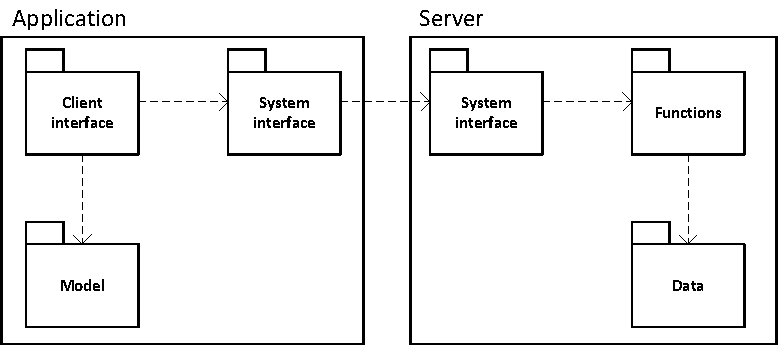
\includegraphics[width=0.9\linewidth]{img/components.pdf}
\caption{System architecture.}
\label{fig:architecture}
\end{figure}

\autoref{fig:architecture} shows the architecture of the entire system. The mobile application has a client interface, for example when a user wants to view a recipe, a request is made through the application's system interface which then receives the recipe data from the server. The recipe data is mapped to the model which can easily be displayed on the device's screen. The application does not have a Functions component because the functionalities are provided by the server.

The server handles requests from clients with its function component. The function component gets the requested data from the database and is then encoded to \ac{json} so the application can easily unsearialise it.